\appendix
\section{Static Oracle: All Evaluated Configurations}
\label{app:oracle}

\Cref{fig:scatterpy,fig:scatter8} complete \cref{fig:scatter}: every fixed configuration the per-core oracle evaluated
for UCP+Pythia on 4 cores and for UCP+IPCP on 8 cores at 2.4\,GB/s per core.  \Cref{tab:oracle4mix,tab:oracle8mix}
list the per-mix results.

\begin{figure*}[!htbp]
\centering
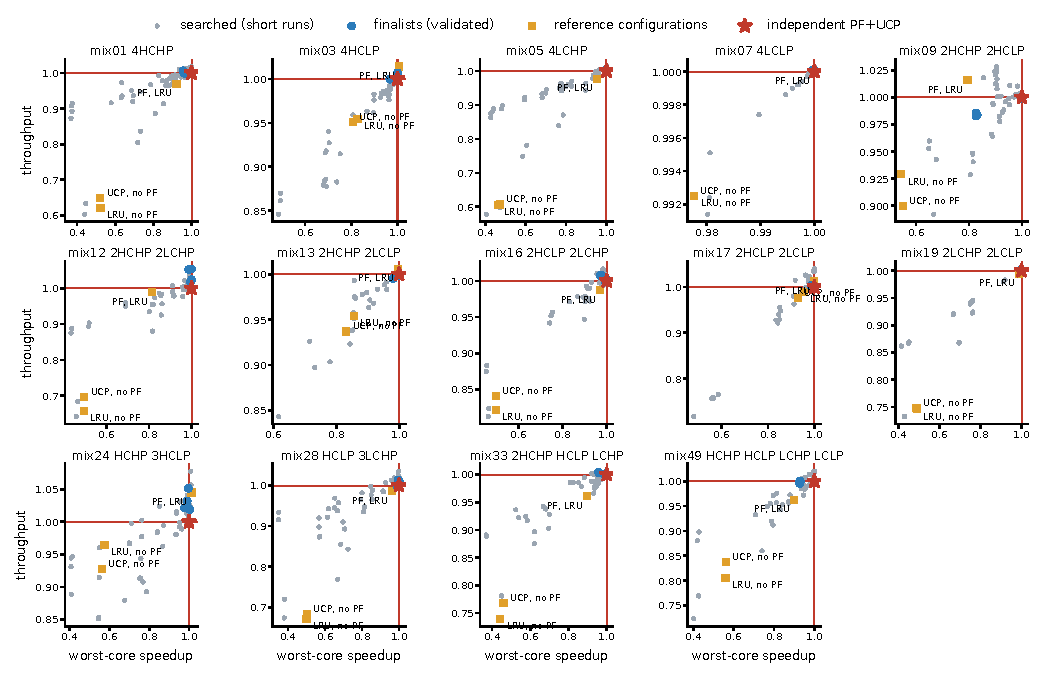
\includegraphics[width=0.9\textwidth]{oracle_scatter_pythia.pdf}
\caption{Per-core static oracle, 4-core, 9.6\,GB/s/core, UCP+Pythia (axes and marks as in \cref{fig:scatter}).}
\label{fig:scatterpy}
\end{figure*}

\begin{figure*}[!htbp]
\centering
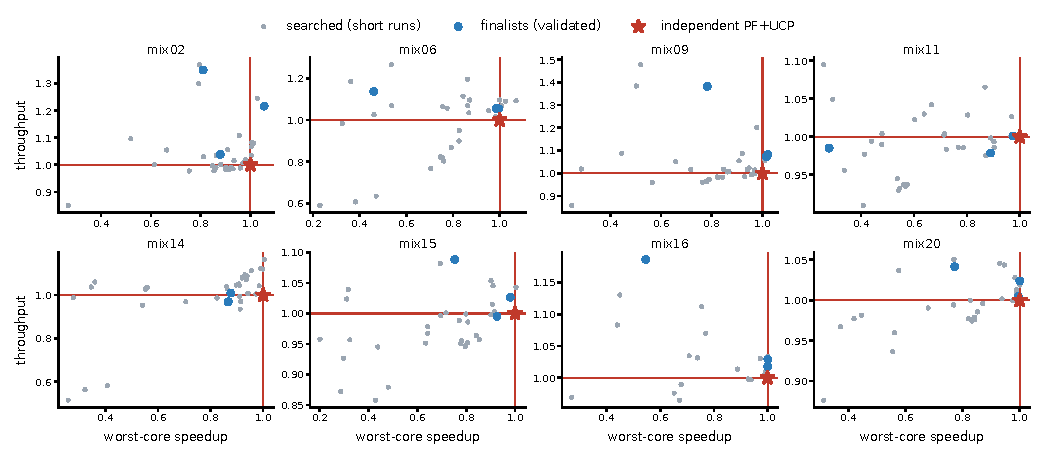
\includegraphics[width=0.95\textwidth]{oracle_scatter_8core.pdf}
\caption{Per-core static oracle, 8-core UCP+IPCP at 2.4\,GB/s/core, axes as in \cref{fig:scatter}.  Many
configurations gain throughput, but the largest gains mostly lie to the left of the star: they sacrifice a core.}
\label{fig:scatter8}
\end{figure*}

\begin{table*}[!htbp]
\centering
\caption{Per-core static oracle, 4-core, 9.6\,GB/s/core: per mix, the best throughput found at the search length when
searching only the prefetch knob, only the partition or both, and the best and the fairest configuration that does not
lose throughput after validation at full length.  Throughput (Thr.) and worst core are relative to independent
operation.  Configuration: ``UCP'' = UCP's adaptive ways, ``ways a/b/c/d'' = fixed ways per core; c$k$ = core $k$,
``cap $d$'' = degree cap $d$, ``off'' = prefetcher off, unlisted cores native.}
\label{tab:oracle4mix}
\footnotesize
\resizebox{\textwidth}{!}{\begin{tabular}{llccclcclcc}
\toprule
 & & \multicolumn{3}{c}{Search length: best of} & \multicolumn{3}{c}{Best validated (throughput)} & \multicolumn{3}{c}{Fairest validated, no throughput loss} \\
\cmidrule(lr){3-5}\cmidrule(lr){6-8}\cmidrule(lr){9-11}
PF & Mix & PF knob & Partition & Both & Configuration & Thr. & Worst & Configuration & Thr. & Worst \\
\midrule
IPCP & 1 & 1.002 & 1.016 & 1.012 & ways 6/1/2/7 & 0.999 & 0.989 & ways 6/1/2/7; c0 cap 4 & 0.999 & 0.991 \\
IPCP & 3 & 1.159 & 1.001 & 1.111 & UCP; all off & 1.172 & 1.074 & UCP; all cap 1 & 1.165 & 1.079 \\
IPCP & 5 & 1.041 & 1.022 & 1.054 & UCP; c1 cap 1 & 1.028 & 1.012 & ways 1/6/1/8; c1 cap 1 & 1.026 & 1.013 \\
IPCP & 7 & 1.000 & 1.000 & 0.999 & UCP; c1 cap 2 & 1.000 & 1.000 & ways 1/5/7/3 & 1.000 & 1.000 \\
IPCP & 9 & 1.119 & 1.042 & 1.019 & UCP; c0 off & 1.108 & 1.010 & UCP; c0 off & 1.108 & 1.010 \\
IPCP & 12 & 1.036 & 1.002 & 1.054 & ways 1/1/1/13; c3 cap 1 & 1.072 & 1.012 & ways 3/1/1/11; c3 cap 1 & 1.051 & 1.013 \\
IPCP & 13 & 1.030 & 0.952 & 1.012 & UCP; c0 cap 1, c2 cap 1 & 1.028 & 1.002 & UCP; c2 off & 1.024 & 1.002 \\
IPCP & 16 & 1.055 & 1.018 & 1.047 & UCP; c0 cap 1, c2 cap 1 & 1.049 & 1.008 & UCP; c0 cap 1, c2 off & 1.049 & 1.010 \\
IPCP & 17 & 1.006 & 1.042 & 1.047 & ways 4/1/1/10; c3 cap 2 & 1.006 & 0.998 & ways 4/1/1/10; c3 cap 2 & 1.006 & 0.998 \\
IPCP & 19 & 1.016 & 1.008 & 1.019 & ways 4/4/4/4; c1 cap 4, c2 cap 4, c3 cap 4 & 1.007 & 0.994 & ways 6/5/1/4 & 1.002 & 1.000 \\
IPCP & 24 & 1.079 & 1.022 & 0.932 & UCP; c0 off & 1.087 & 1.003 & UCP; c0 off & 1.087 & 1.003 \\
IPCP & 28 & 1.078 & 1.067 & 1.100 & ways 1/1/5/9; c3 off & 1.057 & 1.013 & ways 1/1/5/9; c3 off & 1.057 & 1.013 \\
IPCP & 33 & 1.017 & 1.008 & 0.969 & UCP; all cap 4 & 1.036 & 0.962 & UCP; c3 cap 2 & 1.010 & 1.000 \\
IPCP & 49 & 1.003 & 1.024 & 1.025 & ways 1/1/1/13; c1 cap 2 & 0.991 & 0.890 & ways 1/1/1/13; c1 cap 2 & 0.991 & 0.890 \\
\midrule
Pythia & 1 & 0.993 & 1.018 & 1.014 & ways 2/1/1/12 & 1.006 & 0.956 & ways 2/1/1/12; c1 cap 4 & 1.003 & 0.957 \\
Pythia & 3 & 0.994 & 1.000 & 0.886 & UCP; c1 off & 1.007 & 1.000 & UCP; c1 off & 1.007 & 1.000 \\
Pythia & 5 & 1.001 & 1.013 & 1.012 & ways 1/7/1/7 & 1.004 & 0.997 & ways 1/7/1/7; c1 cap 1 & 1.000 & 1.000 \\
Pythia & 7 & 1.000 & 1.000 & 0.999 & ways 1/3/11/1 & 1.000 & 1.000 & ways 1/7/7/1 & 1.000 & 1.000 \\
Pythia & 9 & 1.018 & 1.024 & 1.028 & UCP; c1 cap 2 & 1.001 & 1.000 & UCP; c1 cap 2 & 1.001 & 1.000 \\
Pythia & 12 & 1.017 & 1.018 & 1.032 & ways 1/2/1/12; c1 cap 4 & 1.054 & 0.999 & ways 1/2/1/12 & 1.023 & 1.000 \\
Pythia & 13 & 1.000 & 0.993 & 0.938 & UCP; c0 cap 4 & 1.000 & 0.999 & UCP; c0 cap 4 & 1.000 & 0.999 \\
Pythia & 16 & 1.003 & 1.015 & 1.016 & ways 6/8/1/1; c2 cap 2 & 1.008 & 0.971 & UCP; c2 cap 4 & 1.001 & 1.000 \\
Pythia & 17 & 1.002 & 1.039 & 1.040 & ways 3/1/1/11; c1 cap 4 & 1.004 & 0.987 & ways 3/1/1/11; c1 cap 4 & 1.004 & 0.987 \\
Pythia & 19 & 1.001 & 1.003 & 1.003 & ways 7/5/1/3; c2 cap 4 & 1.002 & 0.997 & ways 7/5/1/3 & 1.000 & 1.000 \\
Pythia & 24 & 1.025 & 1.042 & 1.078 & ways 6/8/1/1; c0 off & 1.052 & 0.996 & UCP; c0 off & 1.019 & 1.004 \\
Pythia & 28 & 1.011 & 1.025 & 1.035 & ways 3/1/1/11; c3 off & 1.014 & 0.996 & UCP; c3 off & 1.011 & 1.001 \\
Pythia & 33 & 1.002 & 1.002 & 1.006 & ways 12/1/1/2; c3 cap 2 & 1.004 & 0.956 & UCP; c0 cap 4 & 1.001 & 0.993 \\
Pythia & 49 & 1.003 & 1.020 & 1.020 & ways 1/1/1/13 & 1.000 & 0.930 & ways 1/1/1/13 & 1.000 & 0.930 \\
\bottomrule
\end{tabular}
}
\end{table*}

\begin{table*}[!htbp]
\centering
\caption{Per-core static oracle, 8-core UCP+IPCP, 2.4\,GB/s/core: per mix, the best and the fairest configuration
that does not lose throughput after validation (notation as in \cref{tab:oracle4mix}), and the search summary.}
\label{tab:oracle8mix}
\footnotesize
\begin{tabular}{rlccclcc}
\toprule
 & \multicolumn{4}{c}{Best validated (throughput)} & \multicolumn{3}{c}{Fairest validated, no throughput loss} \\
\cmidrule(lr){2-5}\cmidrule(lr){6-8}
Mix & Configuration & Knob & Thr. & Worst & Configuration & Thr. & Worst \\
\midrule
2 & UCP; all off & prefetch only & 1.350 & 0.810 & UCP; all cap 2 & 1.216 & 1.055 \\
6 & UCP; all off & prefetch only & 1.137 & 0.461 & UCP; c1 off & 1.053 & 0.996 \\
9 & UCP; all off & prefetch only & 1.382 & 0.783 & UCP; c1 off & 1.082 & 1.021 \\
11 & UCP; c4 cap 2 & prefetch only & 1.001 & 0.975 & UCP; c4 cap 2 & 1.001 & 0.975 \\
14 & ways 1/1/4/6/1/1/1/1 & partition only & 1.009 & 0.877 & ways 1/1/4/6/1/1/1/1 & 1.009 & 0.877 \\
15 & UCP; c2 off & prefetch only & 1.089 & 0.753 & UCP; c6 off & 1.027 & 0.980 \\
16 & UCP; all off & prefetch only & 1.186 & 0.546 & UCP; c1 off & 1.029 & 1.001 \\
20 & UCP; all cap 2 & prefetch only & 1.041 & 0.772 & UCP; c7 cap 2 & 1.024 & 1.000 \\
\midrule
\multicolumn{8}{l}{Search length, mean of the best per mix: prefetch knob only 1.198, partition only 1.044, both knobs 0.976} \\
\multicolumn{8}{l}{Configurations evaluated in total over the 8 mixes: prefetch only 144, partition only 88, both knobs 16} \\
\bottomrule
\end{tabular}

\end{table*}
